\section{Dataset}

%\junwen{Joshua, feel free to structure in your own way for this section. The general structure of presenting the dataset could be: 1) Describe weather, land surface, soil , crop. How they are collected and what preprocess did you take (like how 4x4km aggregated to 1 county). Point out which features change over time and which don't, and explain. 2) remember to properly cite corresponding papers, espeically for sources. If you think the ones I cite here are good, you can keep them, but feel free to find alternatives. 3) after the description, give several interesting plots or analysis in this section, like the ones you presented to Ariel. Plots should better be interesting and hopefully supportive to our claims/methods/results. 4) Properly point out how our dataset is better than the dataset from cnn-rnn paper (nation-wide vs corn belt, more climatic factors?, ours is more complete?) \textbf{1-1.5 pages including figures}}

% \textbf{TODO - add some more details, check citations, add figure, compare with previous dataset}

We collect county-level climate and soil quality features for nearly all of the counties in the US mainland ($3107$ counties in total\footnote{The only exception is Nantucket County, Massachusetts, where land surface model data is entirely missing, since it is an offshore island.}), for 39 years (1981 to 2019, inclusive). To the best of our knowledge, this is the most comprehensive dataset that is publicly available for crop yield prediction. For example, \cite{khaki2020cnn} provide a large-scale dataset, but they only include 13 states across the US Corn Belt, while our dataset covers all 48 states in the contiguous United States. In addition, our dataset includes new features such as soil moisture and soil texture type that were not incorporated into previous datasets.

To ensure feature quality, we collect the features from multiple reliable publicly-available sources. Our ground-truth crop yields are collected from USDA \cite{usda2013national}. Weather factors such as precipitation, temperature, vapor are gathered from PRISM climate mapping system \cite{daly2013prism}. North American Land Data Assimilation System (NLDAS) \cite{xia2012continental} further provides land surface features, such as soil moisture. Additional soil quality features such as pH and sand percentage can be acquired from Gridded Soil Survey Geographic Database (gSSURGO) \cite{soil2019gridded}. More details are provided below.

%Note that the time-dependent features (weather and land surface) are available at a daily time-scale, and we provide a daily dataset. However for this paper's experiments, we aggregate these features to weekly to make our model more computationally tractable.

\junwen{In our \textit{USCrop} dataset, the time-dependent variables are collected and preprocessed to weekly-based features to facilitate a more computationally tractable training.} 

\subsection{Weather}

We collect seven weather variables from the PRISM dataset \cite{daly2013prism}; precipitation, mean dewpoint temperature, maximum temperature, mean temperature, minimum temperature, maximum vapor pressure deficit, and minimum vapor pressure deficit. The dataset is available at a $4 \times 4$ km resolution, every day. To aggregate each feature to the county level, we follow the procedure used in \cite{ortiz2021anthropogenic} and other works. For each county, we compute the weighted average of the variable over all PRISM grid cells that overlap with the county. Each grid cell is weighted by the percentage of the cell that lies inside the county, multiplied by the percentage of that grid cell which is cropland, pasture, or grassland. We used the National Land Cover Database \cite{nlcd} dataset, which is available at a 30m resolution, to compute the percentage of each cell that is covered by cropland, pasture, or grassland. Figure \ref{aggregating_to_county} shows an example of the process we use to aggregate gridded features to the county level.

% first compute a sparse ``weight'' matrix that specifies for each county, 


\subsection{Land Surface}

The North American Land Data Assimilation System (NLDAS) \cite{xia2012continental} is a large-scale land surface model that closely simulates land surface parameters. We collect 16 features from this dataset, including several ``forcing'' weather variables, as well as soil moisture, moisture availability, and soil temperature at multiple soil depths. These data are originally available at a $0.125 \times 0.125$ degree (roughly $14$ km) spatial resolution, and an hourly temporal resolution. We aggregate the hourly data to daily, and aggregate the grid to the county level in the same way as PRISM. 

\begin{figure}[t]
\centering
\includegraphics[width=0.75\columnwidth]{figs/nldas.png}
\includegraphics[width=0.75\columnwidth]{figs/nldas_SOILM_layer1_19810101_county.png}
\caption{Example of aggregating features to county level. \\
\textbf{(a)} raw raster of soil moisture from NLDAS. \\
\textbf{(b)} Percentage cropland/grassland/pasture (used to compute grid cell weights).\\
\textbf{(c)} the county-level values we generated. \textbf{make bigger, make size of figures consistent}}
\label{aggregating_to_county}
\end{figure}

\subsection{Soil Quality}

The gSSURGO dataset \cite{soil2019gridded} provides abundant survey-collected features regarding the soil composition and quality of an area. These gridded features are available at a 30-meter spatial resolution, and \emph{do not change over time}.

In particular, given the raw sand, silt, and clay percentages, we compute the ``soil texture type'' of each pixel based on the Natural Resources Conservation Service Soil Survey's classification scheme \cite{soiltexture}. After this, we have a total of 20 variables that are depth-dependent (so there are values for 6 different soil depth levels), and 6 variables which are the same across all depths. Again, we aggregate these features to the county level using the weighted-average technique, only considering pixels that are cropland/grassland/pasture.

\subsection{Crop Yields}

The USDA Crop Production Reports \cite{usda2013national} provide comprehensive survey-based data on crop yields (measured in bushels per acre) for numerous crops at the county level. Due to budget limitations, not all counties report data in every year, but the data is still quite comprehensive. For example, for corn, all years between 1981 and 2003 have over 2,000 counties across $41$ states reporting data. We have extracted county-level yields for two crops: corn, soybean. 

%Figure \ref{yields_over_time} illustrates how the number of counties with data have changed over time. While there is a decreasing trend, coverage is still high for the core crop-producing counties.

\junwen{We do not have to include Fig. 2 (even in supp). If we have to, then 2020 shouldn't be included. Three subplots in Fig. 1 should have same sizes, legends, and the plots can be bigger. In the current version, Fig.1 also has never been mentioned.}

\joshua{Sure, I removed Figure 2 (plot of number of counties with crop yield data over time). It's non-trivial to fix Figure 1 since plot (c) was plotted with a different R library, but I will try to fix it. I added a mention of Figure 1.}


% \begin{figure}[t]
% \centering
% 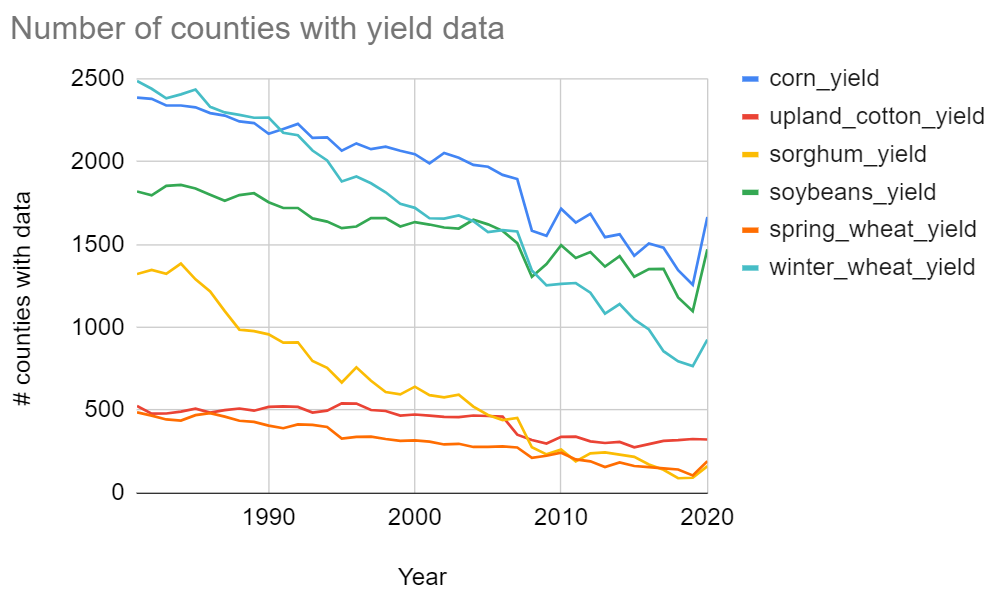
\includegraphics[width=0.8\columnwidth]{figs/counties_with_yield.PNG}
% \caption{Number of counties with yield data over time, for the 6 crops in our dataset. \emph{(this could be moved to Supplemental if it's not critical)}}
% \label{yields_over_time}
% \end{figure}
